
\documentclass{article}

\usepackage{bm}
\usepackage{hyperref}
\usepackage{graphicx}
\usepackage{subcaption}
\usepackage{amsmath,amsthm,amsfonts,amssymb}
\usepackage[latin1, utf8]{inputenc}
\usepackage[dvipsnames,svgnames,x11names]{xcolor}


\title{Lateral remobilization of NSC in the stem wood of tropical trees, reveal high reliability on NSC storage for species with living fibers\\
 }
\author{David Herrera Ramirez \\ Max Planck Institute for Biogeochemistry}

\begin{document}
\maketitle


\begin{abstract}
%\noindent

Trees store large quantities of nonstructural carbon (NSC, mainly sugars and starch) in the stem wood for long periods of time to boost metabolism and growth. 
This NSC is not evenly distributed in the stem wood of mature trees. 
It can also be concentrated in different cell types, for example in ray parenchyma or dispersed in wood fibers.
For many species, NSC concentration decreases radially with sapwood depth.
This gradiente of NSC has to be mobilized when mtabolic demands of carbon are bigger than photosynthesis. 
Wood anatomical characteristics are diverse in tropical trees and they may impose physical constraints on how fast and frequently trees can mobilize NSC stored in stems, having consequences in the survival of trees when facing stressful conditions. 

Here we focus on the following questions: iii) how NSC is remobilized across the radial gradient where it is stored in the stem wood for trropical trees with contrastion sotorage strategies? and iv) how old is the NSC that trees use in respiration under stressful conditions?

To answer these questions we measured NSC content through a radial path in the sapwood (from bark to pith) in 8 tropical tree species in a seasonal dry forest in Brazil during 2018 and 2019. Additionally, we measured the $^{14}$C in the soluble carbon extracted from wood segments corresponding to two depth ranges of each radial path (0-2cm and 2-4cm) and in the respired CO$_{2}$ from 6cm wood core segments. We also estimated the age of the wood core segments by counting annual tree rings and measuring $^{14}$C in the tree ring cellulose.

We found significant seasonal changes in the starch content at different sapwood depths in all trees evaluated, indicating that NSC is metabolically active and remobilized  across all sampled depth ranges. 
%Therefore, we infer that stored C regulates sink activity, reducing the imbalances in carbon sources and sinks. 
%Proportionally, seasonal changes were larger for species that store starch dispersed in wood living fibers. 
Some of these trees stored NSC in the wood for decades, but fiber storing species store NSC for longer time than parenchyma storing species. 
In some cases NSC was even older than the wood that contained it, indicating that these trees maintain the radial pattern of NSC concentration by a predominantly outward mixing of old NSC from deeper layers of wood. 
Irrespective of how old the NSC extracted from the wood was, trees always used younger NSC for respiration. 
However, the respired CO$_{2}$ got older during the dry season, when trees faced a reduction in photosynthesis and may have entered a negative C balance requiring a larger contribution of old stored NSC to respiration.

%These findings highlight the high diversity of storage strategies in tropical trees that may be tightly linked to the ability of those trees to survive stressful conditions. 
These results have important implications for our understanding not only of how trees will respond to future climatic changes but also about the mechanisms of carbon cycling in tropical trees.


\end{abstract}

\section{Introduction}

Trees assimilate $CO_{2}$ into non-structural carbon (NSC), which is mainly soluble sugars, starch and lipids. 
Non-structural carbon is transported to and accumulated in all tree organs to fuel metabolism and growth at different time scales, from seasonal to inter-annual. 
Changes in the quantity of NSC indicate the carbon status and the imbalances between carbon sources (e.g. photosynthesis) and sinks (e.g. growth and respiration) in trees. Additionally, 
NSC also serves in maintaining and repairing hydraulic conditions within tree stems. Thus, NSC dynamics indicate the tolerance of trees to disturbances or stress. 
Understanding how NSC dynamics vary between tree species would help us to estimate what trees would have higher tolerance to future climatic changes. 

Stem-wood plays a central role in NSC dynamics and long term storage for mature trees. 
Quantification of NSC across sapwood at different depths has shown a decreasing pattern of NSC concentrations with sapwood depth. 
The shape of this radial pattern varies among species and it is related to wood anatomy. 
It has been shown that wood anatomical traits as porosity distribution constrain not only the NSC distribution in wood, but also its seasonal cycling in temperate trees.
 Previous work has reported diffuse porous species to have lower concentration of NSC, deeper storage and lower seasonal activity than ring-porous species. 
 Another functional trait that control the shape of the radia distribution of starch in the stemwood is the presence of living fiber
 Traditionally, it has been thought that these seasonal fluctuations are mainly controlled by sink activity. 
 Stressful conditions as drought or low temperature reduce growth and respiration stronger and faster than they do to photosynthesis, leading trees to accumulate NSC. 
 Nevertheless, it has also been reported that under mild stressful conditions as mild droughts or disturbances NSC fluctuations in the stem-wood can be controlled by source activity.
 
these traits may induce strong differences in the seasonal and multianual fluctuations of the NSC. 
some of these traits would benefit the fast cycling of NSC and the low accumulation of reserves, while other traits (living fibers, difuse porosity, high amount of axial parenchyma, high longevity of living wood cells) would benefit no only larger accumulation of NSC but also the storage of these NSC for longer. 


%For tropical trees there is scarce information to understand what are the seasonal changes in the radial pattern of NSC in the wood, what drives them and how they are related to wood anatomical traits. In several tropical trees a decreasing pattern of NSC content with wood depth has also been reported, but we still can not relate it with any wood anatomical trait or life history trait. Wood anatomical traits as the storage of starch in living fibers seems to play a relevant role in NSC dynamics for tropical trees. In a previous work we showed that the storage strategy related to where starch was stored in the wood determined the storage capacity of some tropical trees and it was related with their growth and mortality rates. Thus, trees that store starch in the living fibers had higher storage capacity, lower growth and lower mortality than trees that did not have living fibers and only store starch in parenchyma cells. We still do not know how this wood storage strategies would be related with seasonal fluctuation of the radial distribution of NSC in the stem wood of tropical trees, the period of time NSC is stored in wood and the ability of trees to access and cycle the stored NSC in deep wood layers.
%

Seasonal fluctuations in the radial pattern of NSC across the sapwood reflect the lateral inward and outward mixing of NSC. Contrary to the NSC concentration in wood, the NSC age increase with depth. 
This means that the outermost layers of wood contain mostly new, recently assimilated, NSC, while deeper layers of wood contain mostly old carbon. 
Radiocarbon measurements have shown that generally stored NSC is always younger than the wood that contains it, demonstrating that the radial pattern of NSC across sapwood is maintain mostly by an inward mixing of new NSC from the phloem to deep layers of wood. 
The strength of this inward mixing vary among species, but there is still no evidence of old NSC mixing out from deep old layers of wood to the superficial new ones. Furthermore, these inward mixing rates are still unclear for tropical trees. 
Revealing these patterns for tropical trees will help us to understand for how long NSC is stored in the wood, how fast it is cycled and how determinant are the wood functional traits for NSC dynamics in these trees.

Previous works have shown that tropical trees store NSC for long periods of time (even decades), and it can be used on respiration and growth following major disturbances or stress. 
Nevertheless, carbon allocated to growth and respiration under favorable conditions is always younger than the NSC stored in the wood. 
This has been explained by the existence of a fast and slow NSC pools in the wood. 
Simulations of NSC ages and transit times has shown us that these NSC dynamics result in asymmetrical NSC age distributions skewed towards young, recently assimilated carbon, which  fuel respiration and growth under favorable conditions. 
When limiting conditions come, trees have consume their NSC stored in the wood, increasing the contribution of old stored NSC to respiration. 


%Here we wanted to test how much seasonal fluctuations in the NSC may be reflected in the age of the respired NSC from stem cores to understand until what extend trees use their reserves under seasonal stressful conditions. For this we compared the age of the NSC stored in the wood with the age of the $CO_{2}$ emitted by that wood (Figure 1). The area under the 1:1 line show this relation. We hypothesized that when trees have to use their storage to survive a major disturbance or a stress, the age of the emitted $CO_{2}$ will increase, moving the ratio $CO_{2} age : NSC age$ closer to 1:1. The more the trees' reserves are used the closer to 1:1  this ratio will be. 

In this work we want to better understand NSC dynamics for tropical trees in a seasonally dry forest in Brazil. For this we measured the seasonal activity of the radial pattern of starch concentration in the wood of species with contrasting wood anatomical traits and we measure the age of the NSC across this radial pattern and the age of the respired $CO_{2}$ directly from  stem-wood cores. We aim to answer the following questions: 
%i) how is the seasonality in the radial distribution of starch concentration in the stem-wood of tropical trees with contrasting wood storage strategies growing in a seasonally dry forest? 
%ii) how this seasonality may be related with the balance between sources and sinks? 
i) how old is the NSC stored in the wood of tropical trees and how is it related with wood functional traits and starch dynamics in the stemwood. 
iii) How in the radial remobilization of NSC across the sapwood for tropical tree species with contrasting wood anatomical traits and 
iv) how old is the NSC that these tropical trees access for respiration, and how much does it change with seasonal stressful conditions? 
%For answering these question we provide a detailed accounting of the spatial and temporal variation of NSC within the stem wood of tropical trees with contrasting wood storage strategies. 
We estimated the mean age of the NSC within the stem wood and the mean age of the respired $CO_{2}$ and the mean age of the wood where the NSC is stored. 


\section{Methods}

\subsection{Site description}

This study was conducted at a transitional forest between the Amazon rainforest and Cerrado, located at Tanguro Ranch, Mato Grosso, Brazil (S \ang{13;04;35.39}, W \ang{52;23;08.85}). It is a seasonal dry forest with mean annual precipitation of 1770mm, a marked dry season between May and September with less than 10mm of precipitation per month, and a wet season between October and April with a mean precipitation of 150mm per month (Fig. \ref{fig:climatic_seasonality}). Relative humidity follows a similar seasonal pattern, falling below 60\% from June to September and greater than 80\% from December to February (Fig. \ref{fig:climatic_seasonality}).  Mean temperature is 25$^{\circ}$C with almost no seasonal variation throughout the year (Data obtained from a local station at Tanguro Ranch operated by the Instituto de Pesquisa Ambiental da Amazônia, IPAM). 


\begin{figure}[h] %  figure placement: here, top, bottom, or page
   \centering
   \begin{subfigure}{0.50\textwidth}
   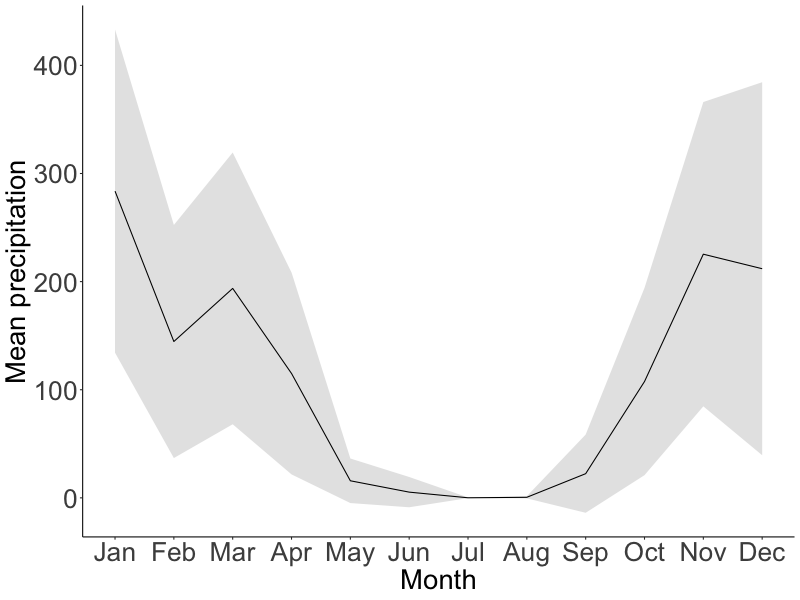
\includegraphics[width=\textwidth]{precipitation_seasonality.png} 
   	\caption{}
          \label{fig:precipitation} 
       \end{subfigure}
	 \begin{subfigure}{0.48\textwidth}
   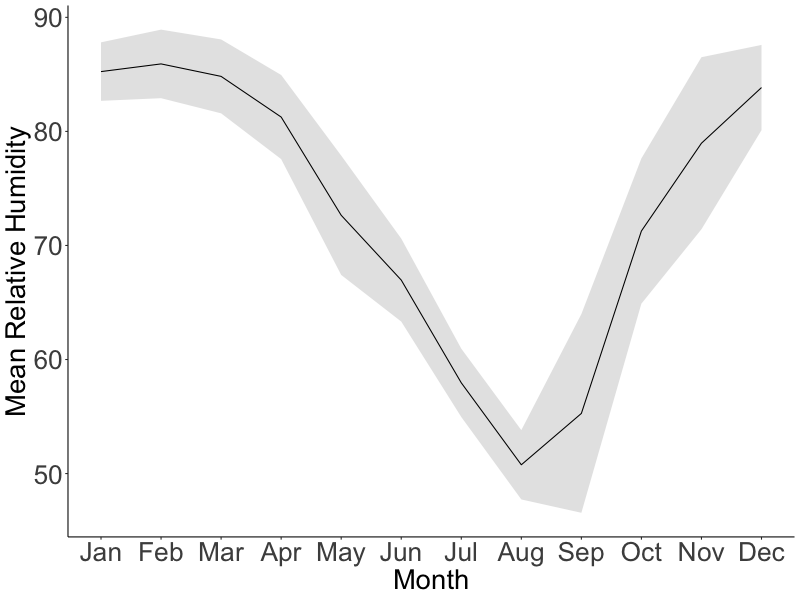
\includegraphics[width=\textwidth]{Relative_humidity_seasonality.png} 
   	\caption{}
          	\label{fig:Relative_humidity} NSC
	\end{subfigure}
   \caption{Mean seasonal course of precipitation (mm) and relative humidity (\%) during 2016-2020 (black lines). Gray areas correspond to the standard deviation. Data provided by IPAM. }
   \label{fig:climatic_seasonality}
\end{figure}	

\subsection{Species description}

We sampled 12 individual trees per species from eight species that demonstrated to have contrasting starch storage strategies in wood \citep{Herrera-remirez:2021}, different leaf habit (evergreen or semi-deciduous) and different growth and mortality rates (Table \ref{tree_species}). From each tree species we chose mature and healthy trees reaching the canopy with a diameter at breast height (at 1.3m, dbh) bigger than 20cm (Table \ref{tree_species}). 

 
\begin{table}[h]
\caption{Species names and traits: wood storage strategy, growth rates, mortality rates, phenology, and the sampling dates.}
\begin{center}
\resizebox{\textwidth}{!}{
\begin{tabular}{  p{4cm} p{2cm} p{2cm} p{3cm} p{3cm} p{3cm} }
\hline
Species name &  Growth rate (cm/yr) & Mortality rate (\%/yr) & Storage strategy & Leaf phenology & Sampling date\\
\hline\hline
\textit{Ocotea leucoxylon} (Sw.) Laness & 0.295 & 5.7 & Parenchyma & Evergreen &  Jan18, Jul18, May19, Aug19, Nov19, Feb20\\
\textit{Ocotea guianensis} Aubl. & 0.282 & 4.1 & Parenchyma & Evergreen & Jan18, Jul18\\
\textit{Sacoglotis guianensis} Benth. & 0.72 & 5 & Parenchyma & Semi-deciduous &  Jan18, Jul18, May19, Aug19, Nov19, Feb20\\
\textit{Vochysia vismiifolia} Spr. Ex Warm. & 1.32 & 3.1& Parenchyma & Semi-deciduous & Jan18, Jul18\\
\textit{Dacryodes microcarpa} Cuart. & 0.078 & 1.6 & Fiber  & Semi-deciduous & Jan18, Jul18, May19, Aug19, Nov19, Feb20\\
\textit{Tapirira guianensis} Aubl. & 0.47 & 2.5 & Fiber & Semi-deciduous & Jan18, Jul18\\
\textit{Trattinnickia burserifolia} Mart. & 0.09 & 1 & Fiber & Evergreen & Jan18, Jul18\\
\textit{Trattinnickia glaziovii} & 0.12 & 1.7 & Fiber & Evergreen & Jan18, Jul18\\
\hline
\end{tabular}
}
\end{center}
\label{tree_species}
\end{table}
 
 
\subsection{Sampling scheme}

We sampled each tree periodically during two years (2018 and 2019). In 2018 we took samples during the wet season, in January, and during the dry season, in July. In January, we randomly sampled 5 individuals per species while in July we resampled the same 5 individuals from January plus 7 new ones also randomly selected, to increase our sampling size to 12 individuals per species. In 2019 we continued sampling the same 12 individuals previously sampled every three months (May 2019, Aug 2019, Nov 2019 and Feb 2020) from a subset of three species that represented our group of species in terms of the starch storage strategy, leaf habit and growth (\textit{Ocotea leucoxylon, Sacoglotis guianensis} and \textit{Dacryodes microcarpa}, Table \ref{tree_species}). 

From each individual tree and sampling event, we extracted three wood cores (5 mm diameter) from bark to pith using an increment borer (Fig. \ref{fig:Sampling_scheme}). The increment cores were taken at the same height (1.3 m), 5 cm apart from each other (horizontally). In the subsequent field campaigns, cores were taken 5 cm away from where the last samples were taken. Two of the cores were placed in ice immediately after collection and frozen at $-18^{\circ}$C within two hours. They were kept frozen until it was possible to dry them in an oven at $60^{\circ}$C for two days. 

We used one of the wood cores to quantify starch along the radial axis of the wood core from bark to pith using the histological method described in \citep{Herrera-remirez:2021} in the Plant Biodiversity Lab in Jena. We quantified starch in the wood cores for every sampling event.

We used the second core to extract the water soluble carbon and starch to measure the soluble sugars concentration and the $^{14}$C signature of the water-soluble carbon and starch. This core was divided in two depth ranges (0-2cm and 2-4cm). We did this measurement only for the cores from July 2018, because we did not expected the age of the NSC stored in the wood to vary significantly between seasons. 
The third wood core was wrapped in a wet tissue immediately after collection and protected from direct sun and extreme heat to maintain it alive. We used the first 6 cm of these cores for collecting the CO$_{2}$ emitted and measuring the respective $^{14}$C signature (Fig. \ref{fig:Sampling_scheme}). We collected the CO$_{2}$ to measure wood core respiration and its $^{14}$C signature in July 2018 and in May 2019. 


 \begin{figure}[h] %  figure placement: here, top, bottom, or page
   \centering
   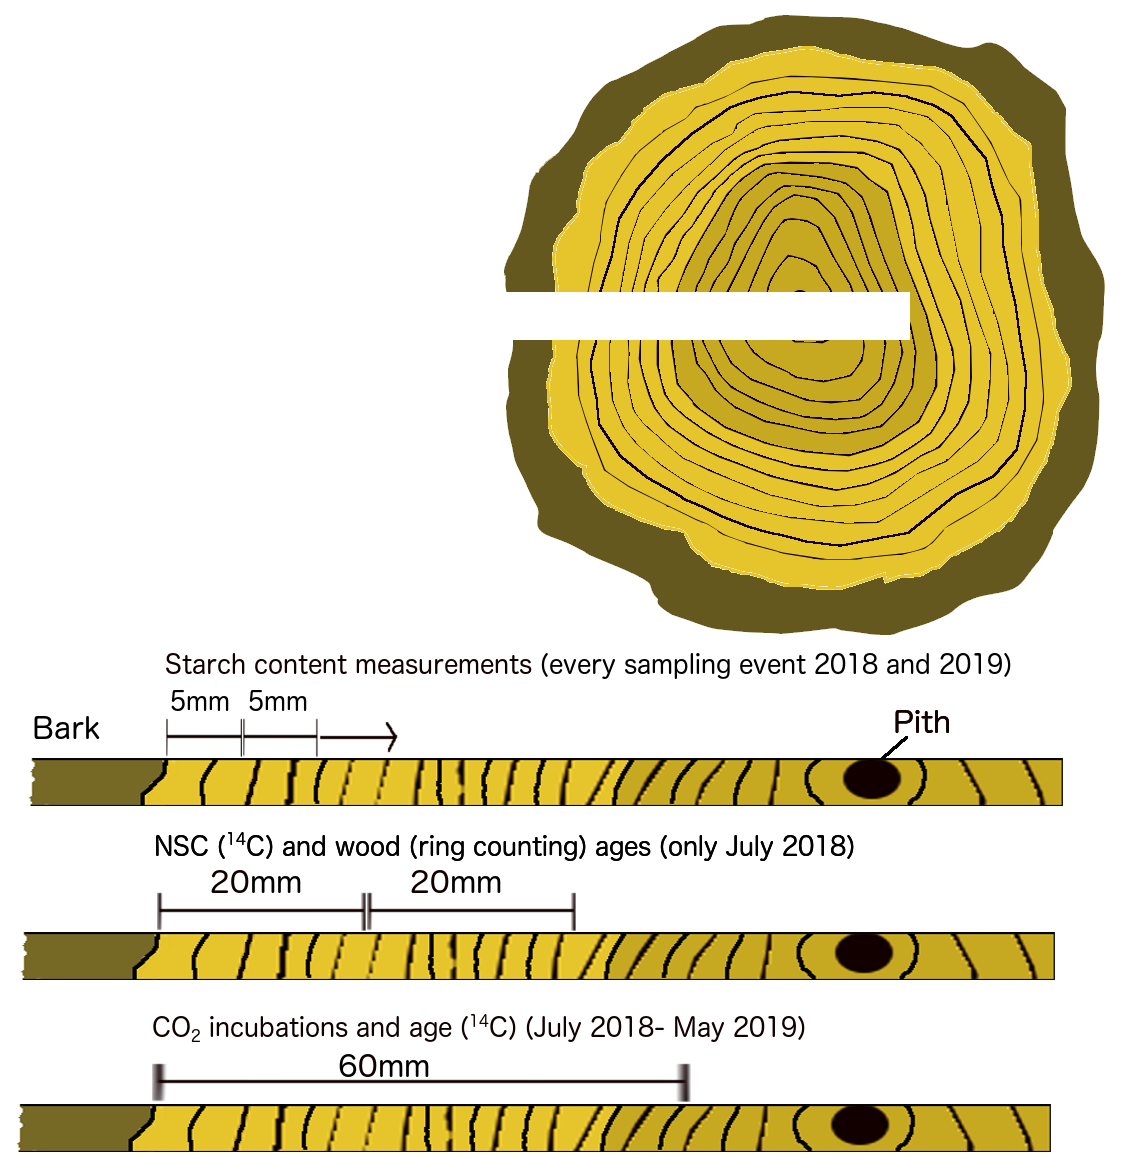
\includegraphics[width=4in]{figure_methods.png} 
   \caption{Specification of the treatments applied for each of te stem wood cores collected from each three and each sampling date. We collected three increment cores from each individual and we used each core for different measurements as specifies in the image. In parenthesis, I specify the sampling dates when the specific measurements were taken.}
   \label{fig:Sampling_scheme}
\end{figure}



\subsection{$^{14}$C signature of the water-soluble carbon and starch} 

The second core was also used for measuring the $^{14}$C signature of the water soluble carbon, which contains a fraction of the soluble sugars stored in the wood. We measured 5 individuals per species from the samples taken in July 2018. We extracted and measured soluble carbon from the first 4 cm of the wood cores, in two depth ranges, from 0 to 2 cm and from 2 to 4 cm. We extracted the soluble carbon from 50 mg of ground samples of each wood core segment produced before. We dried 50 to 100 mg of wood powder at $60^{\circ}$C overnight. Dry samples were boiled in 1.5 ml of distilled carbon-free water for 10 min at $80^{\circ}$C. After cooling to room temperature, the samples were centrifuged at 13000g for 2 minutes. We then collected the supernatant in a new vial. We repeated the process three times, always collecting the supernatant in the same vial. The supernatant was later condensed under vacuum. From this condensed solution we collected aliquots between 0.5 and 2.5 mg into a silver cup, dried in an oven at $60^{\circ}$C, and then processed according to \citet{steinhof:2017} to measure the $^{14}$C signature by Accelerator Mass Spectrometry (AMS) at the Jena $^{14}$C lab. Data are reported as $\delta^{14}$C, which is the per mil deviation from 0.95 times the $^{14}$C/$^{12}$C ratio of oxalic acid standard in 1950 (equivalent to the 1895 wood standard).

The mean age of the carbon was estimated using the radiocarbon calibration curve corresponding to the bomb spike, from 1955 to 2012 \citep{hua:2013}. Samples that had a $\delta^{14}$C value corresponding to the years after 2012 were calibrated using a linear regression fit to the last ten years of the calibration curve \citep{hua:2013}  and a $\delta^{14}$C value measured in the structural carbon of an annual plant in 2019. We assumed this value corresponded to the $^{14}$C signature of carbon fixed from the atmosphere in 2019. Differences in the $\delta^{14}$C between samples reflect the differences in the time since the fixation of CO$_{2}$ from the atmosphere. All radiocarbon data reported as $^{14}$C have been corrected for any variations in mass-dependent isotope fractionation, using the AMS-measured $^{13}$C value and assuming $^{14}$C is fractionated twice as much as $^{13}$C (see \citet{Trumbore2016}).
 
To measure the $^{14}$C of the starch fraction, we extracted starch from the remaining pellet resulting from the water soluble carbon extraction. The pellet was dried overnight at $60^{\circ}$C. We used the enzymatic digestion method described by \citet{Landhausser:2018aa}, but using hot water instead of ethanol. We converted starch into soluble oligosaccharides by adding one ml of alpha-amylase (600 units/ml) from bacillus licheniformis (Sigma cat no A 4551) to the dry pellet. Samples were incubated in an orbital shaker for 1 hr at $85^{\circ}$C. Then the samples were left to cool down to room temperature and centrifuged at 13000g for 3 minutes. The supernatant was transferred to a new 2ml srew-cap microcentrifuge tube. The enzyme was cleaned up from the supernatant with chloroform. Each batch of 45 samples was run along with 3 standards of the sugars (IAEA-C6 with a $\delta^{14}$C~500). The solution was then condensed under vacuum and the oligosaccharides from the starch were then dried in silver cups until harvesting 1mg. To correct for small traces of exogenous carbon coming from the enzyme we use the following model:

\begin{equation}
{\delta^{14}C_{measured}}=\frac{\delta^{14}C_{starch} \cdot Mass_{carbon-starch} + \delta^{14}C_{enzyme} \cdot Mass_{carbon-enzyme}}{Mass_{total}}
\label{starch_mass_balance_eq}
\end{equation}

Where $\delta^{14}C_{measured}$ is the $\delta^{14}$C from the analysed sample. $\delta^{14}C_{starch}$ is the corrected $\delta^{14}$C that we aimed to obtain from Equation \ref{starch_mass_balance_eq}. $Mass_{carbon-starch}$ is the mass of carbon coming from starch in the sample, $\delta^{14}C_{enzyme}$ is the $\delta^{14}$C of the enzyme that we used for the extraction and the $Mass_{carbon-enzyme}$ is the fraction of carbon coming from the enzyme. $Mass_{total}$ is the sum of the mass of carbon from starch and the mass of carbon from the enzyme. The $\delta^{14}C_{measured}$ was directly measured in the sample. The mass of carbon coming from the starch was estimated from the mass of starch measured in the samples and multiplied by the molar mass of carbon in sugars (0.44). The $\delta^{14}C_{enzyme}$ was directly measured from three enzyme samples by AMS. The mass of carbon coming from the enzyme was estimated by multiplying the mass of enzyme used in the extraction by a factor of 0.09, which is the estimated percentage of the carbon from the enzyme remaining in the sample after processing. To estimate the percentage of carbon coming from the enzyme in the sample we measured the $\delta^{14}$C in 18 solutions of the standard sugar (IAEA-C6). We prepared three different groups to test if the concentration of the sugar would affect the contamination from the enzyme, each group consisted of different ratios of sugar/enzyme, 1.5, 0.8 and 0.4 (mg-sugar/mg-enzyme) respectively and 6 samples. We processed these solutions following the same protocols for starch extraction described above, and finally we measured their $\delta^{14}$C with AMS. With these measurements we used Equation \ref{starch_mass_balance_eq} to estimate the percentage of carbon coming from the enzyme after the extraction process. Then we used this value (0.09) in Equation \ref{starch_mass_balance_eq} to correct the $\delta^{14}$C value in our samples. 

\subsection{CO$_{2}$ efflux from wood cores and its $^{14}$C signature}

For sampling of CO$_{2}$ directly emitted by wood, we took an extra wood core sample from each tree from \textit{D. microcarpa, S. guianensis} and \textit{O. leucoxylon}. We collected the CO$_{2}$ by laboratory incubations of increment wood cores of 6 cm long. We did these incubations during the dry season 2018 (July 2018) and the wet season 2019 (May 2019). Gas samples containing the CO$_{2}$ derived from the incubations were collected in custom-built glass flasks (volume: 115ml) equipped with an O-ring valve (Louwers H.V. glass valves, Louwers Glass and Ceramic Technologies, Hapert, Netherlands, 12mm ID) and shipped to the laboratory for further analyses. Stem chambers consisted of a 10 cm long piece of stainless steel tubes with stainless steel fittings on both sides of the tube sealed by a Viton O-ring on each side. Thus, one glass flask could be attached to each side of the chamber. For the incubations, we cut a 6cm segment of each wood core from cambium to pith, we carefully removed the bark from each wood core, and placed the wood core inside of the incubation chamber. The flasks were flushed with CO$_{2}$-free air before attaching to the fittings. Once we attached the flasks and verified that the system was completely sealed, we opened the O-rings on each side of the flasks and left the incubations running at room temperature for 24 hours in July 2018 and 36 hours in May 2019. It was necessary to increase the incubation time in May 2019 due to the very low amount of CO$_{2}$ collected in July 2018 from \textit{O. leucoxylon} and \textit{S. guianensis} trees that did not provide enough carbon to measure the $^{14}$C signature.

We estimated the quantity of CO$_{2}$ respired by each sample in each flask by measuring the pressure at room temperature on a vacuum line. Then we calculated the respiration rate for each sample dividing the total amount of collected CO$_{2}$ in mg by the incubation time. Then, we extracted the CO$_{2}$ cryogenically from each flask and reduced it to graphite to measure the $^{14}$C signature with AMS according to \citet{steinhof:2017}. Here, $^{14}$C data are reported in $\delta^{14}$C and compared with the records from the radiocarbon curve from 1955 to 2012  \citep{hua:2013} to estimate the average year in which the carbon was fixed from the atmosphere. For the samples that had a $\delta^{14}$C from years after 2012 we used the linear fit mentioned above to estimate the $^{14}$C age of the CO$_{2}$


\subsection{Wood age estimation}

We estimated the age of each wood core by counting annual tree rings in 7 of the 8 species studied. For the species (\textit{S. guianensis}) the difference between estimated ages of wood formation based on tree ring counting and $^{14}$C was larger than 5 years (Fig. S1), and therefore tree ring counting was not possible in this species. We validated the ring counting approach by measuring the $^{14}$C in the structural carbon of some tree rings on two randomly selected trees per species. We first counted the number of tree rings in each wood core and assigned dendrochronological ages to each tree ring. Then, we isolated two tree rings per stem core, we ground the wood and extracted the cellulose following the procedures described by \citet{steinhof:2017}. Later, the $^{14}$C was measured in the cellulose of each tree ring. We expressed the $^{14}$C as fraction modern (FM) and compared it directly with the radiocarbon calibration curve from 1955 to 2012 \citep{hua:2013} to estimate the year of wood formation \citep{Andreu-Hayles:2015wb}. Then, we compared the dendrochronological age of the tree ring with the year of wood formation estimated by $^{14}$C. This analysis allowed us to identify the species on which we could estimate the wood age by tree ring counting with an uncertainty of  5 years (Fig. S1). Then we estimated the average age of each 2 cm wood core segment for each tree by averaging the age of the tree rings contained in each segment. We did not find differences between the estimation of the wood mean age by an arithmetic average of the tree ring ages and a weighted average of the tree ring ages using width as a weight (Fig. S2), therefore we used the average of tree ring ages in a wood core section to estimate the mean wood age of each wood core section.

For trees from \textit{S. guianensis} we estimated the mean age of each 2 cm segment of wood core from the $^{14}$C in the cellulose. We took 20 mg of ground wood from each wood core segment and extracted the cellulose following \citet{steinhof:2017}. Then we estimated the mean age based on the $^{14}$C measurements for each wood core segment using the radiocarbon calibration curve of the bomb spike \citep{hua:2013}.


\subsection{Stem diameter growth rates}

Stem growth rates were recorded from manual dendrometer bands (D1, Labcell Ltd, UK) installed in trees of the three species measured during 2019 (see Table \ref{tree_species}). Dendrometer bands were installed in 10 trees per species at 1.3m in July 2018, and measurements were collected monthly until July 2020. Measurements were collected manually by direct reading of the dendrometer bands.
 
 \subsection{Data analysis}
 
We used ANOVAs for all statistical comparison between groups of measurements that had normal distribution of the residuals such as starch concentration and content between seasons and species, respiration rates between trees species and seasons, $\delta^{14}$C of the NSC between storage strategies, leaf habit, and species, and $\delta^{14}$C of the CO$_{2}$ emitted by the stem cores between species.

To evaluate the effect of changes in the radial gradient of starch concentration in the wood cores we used a nonlinear mixed effect model. We modelled the radial distribution of starch in the wood core by the nonlinear model (Equation \ref{starch_area_nlm}). Then we estimated the model parameters using months as a random variable. We compared the random effect of the measurement months with the fixed effects to estimate the seasonal variability on the model parameters. 
 

\begin{equation}
\mathrm{Starch \ area} \%= \exp(a+b*log(depth)+c*depth).
\label{starch_area_nlm}
\end{equation}

We also evaluated the seasonal changes in the radial gradient of the starch content by estimating the absolute and relative seasonal amplitude of the starch concentration in each of the 5 mm radial increments of the wood core where the starch concentration was measured during the year 2019. We estimated the seasonal amplitude for each wood segment as the maximum starch concentration minus the minimum starch concentration of the year 2019. Relative changes were calculated with respect to the maximum starch content of 2019. We calculated a mean curve per species and its standard deviation using all 12 measured trees per species. The significance of these changes was evaluated with ANOVAs.

In order to compare the age of the NSC with the age of the structural wood that contained it, we estimated linear regression models between the soluble carbon $\delta^{14}$C mean age and the wood core mean age (estimated by tree ring counting) for each species grouped between storage strategies and leaf habit. 



\section{Results}

\subsection{Seasonality of starch content and its radial distribution in the stem wood of 9 tropical trees}

Starch concentrations followed a decreasing pattern radially across sapwood from bark to pith for all species in all sampling dates, except for \textit{V. vismiifolia} that showed no significant change in the NSC concentration with sapwood depth (Fig. \ref{fig:starch_radial_pattern}, Table \ref{Nonlinear_mix_models}). This radial pattern of starch in the wood varied between species and between sampling dates (Fig. \ref{fig:starch_radial_pattern} and  \ref{fig:starch_radial_activity} , Table \ref{Nonlinear_mix_models}). For instance, some trees of \textit{V. vismiifolia}, that store starch only in the parenchyma and grow very fast (around 1cm/year), had almost no starch stored in the wood and show constant and close to zero levels of starch across all wood cores (Fig. \ref{fig:starch_radial_pattern}); others ( \textit{O. leucoxylon} and \textit{O. guianenesis}) had very shallow starch storage that decreased in concentration very quickly within the first 4 cm of wood, and still others ( \textit{S. guianensis}) had constant concentration of starch over the first 6cm of wood before it started to decrease slowly, reaching wood depths up to 12 cm (Fig. \ref{fig:starch_radial_pattern}). For species that store starch in the living fibers the situation was similar. Some trees (\textit{T. guianensis}) showed storage that decreased within the first 5 cm of wood, while others ( \textit{D. microcarpa, T. burserifolia} and \textit{T. glaziovii}) showed a peak of starch concentration around 2cm of wood depth followed by a gradual decrease within the next 7 cm of wood (Fig. \ref{fig:starch_radial_pattern}). After these depth thresholds wood was completely devoid of starch in all trees investigated.

\begin{table}[h]
\caption{Statistics for the nonlinear mixed models in Equation \ref{starch_area_nlm} fitted for each species with the sampling date as a random effect. The value ``All'' in the sampling date evaluated stands for all sampling dates (Jan18, Jul18, May19, Aug19, Nov19 and Feb20). 0.05 significance of the fixed effect parameters is indicated by *, 0.01 by **, and 0.001 by ***; n.s. stands for not significant and n.e. stands for not estimated. Here we show the Bayesian Information Criterion (BIC), the sampling dates that were used in the model, the random effects standard deviation of each parameter and the standard error for each parameter of the fixed effects. 
}
\begin{center}
\resizebox{\textwidth}{!}{
\begin{tabular}{  p{4cm} p{2cm} p{2cm} p{1cm} p{1cm} p{1cm} p{1.5cm} p{1.5cm} p{1.5cm} }
\hline
Species name &  BIC & Sampling date evaluated & \multicolumn{3}{p{3cm}}{Random effect standard deviation (Sampling date)} & \multicolumn{3}{p{4.5cm}}{Fixed effects standard errors (depth)}\\
\hline\hline
 & & & a & b & c & a & b & c \\
\textit{Ocotea leucoxylon} & 2397 & all &0.39 &0.13 & 0.006 & 0.005*** & 0.008*** & 0.004***\\
\textit{Sacoglotis guianensis} & 6623 & all & 0.52 & 0.18 & n.e. & 0.26*** & 0.1*** & 0.002***\\
\textit{Dacryodes microcarpa}& 4212.1 & all & 0.62 & 0.25 & n.e. & 0.32* & 0.16*** & 0.009***\\
\textit{Ocotea guianensis} & 468 & Jan18-Jul18 & 0.17 & 0.60 & 0.06 & 1.05* & 0.86** & 0.08***\\
\textit{Trattinnickia glaziovii} & 1302 & Jan18-Jul18 & 0.27 & 0.02 & 0.01 & 0.38** & 0.21*** & 0.01***\\
\textit{Trattinnickia burserifolia} & 934.8 & Jan18-Jul18 & 0.19 & 0.84 & 0.06 & 0.62** & 0.65* & 0.04 n.s.\\
\textit{Tapirira guianensis} & 627.2 & Jan18-Jul18 & 0.74 & 0.60 & 0.04 & 0.68** & 0.52 n.s. & 0.03***\\
\textit{Vochysia vismiifolia} & n.e. & Jan18-Jul18 & n.e. & n.e. & n.e. & 2.3 n.s & 1.86 n.s. & 0.14 n.s.\\
\hline
\end{tabular}
}
\end{center}
\label{Nonlinear_mix_models}
\end{table}
 

 \begin{figure}[p] %  figure placement: here, top, bottom, or page
   \centering
   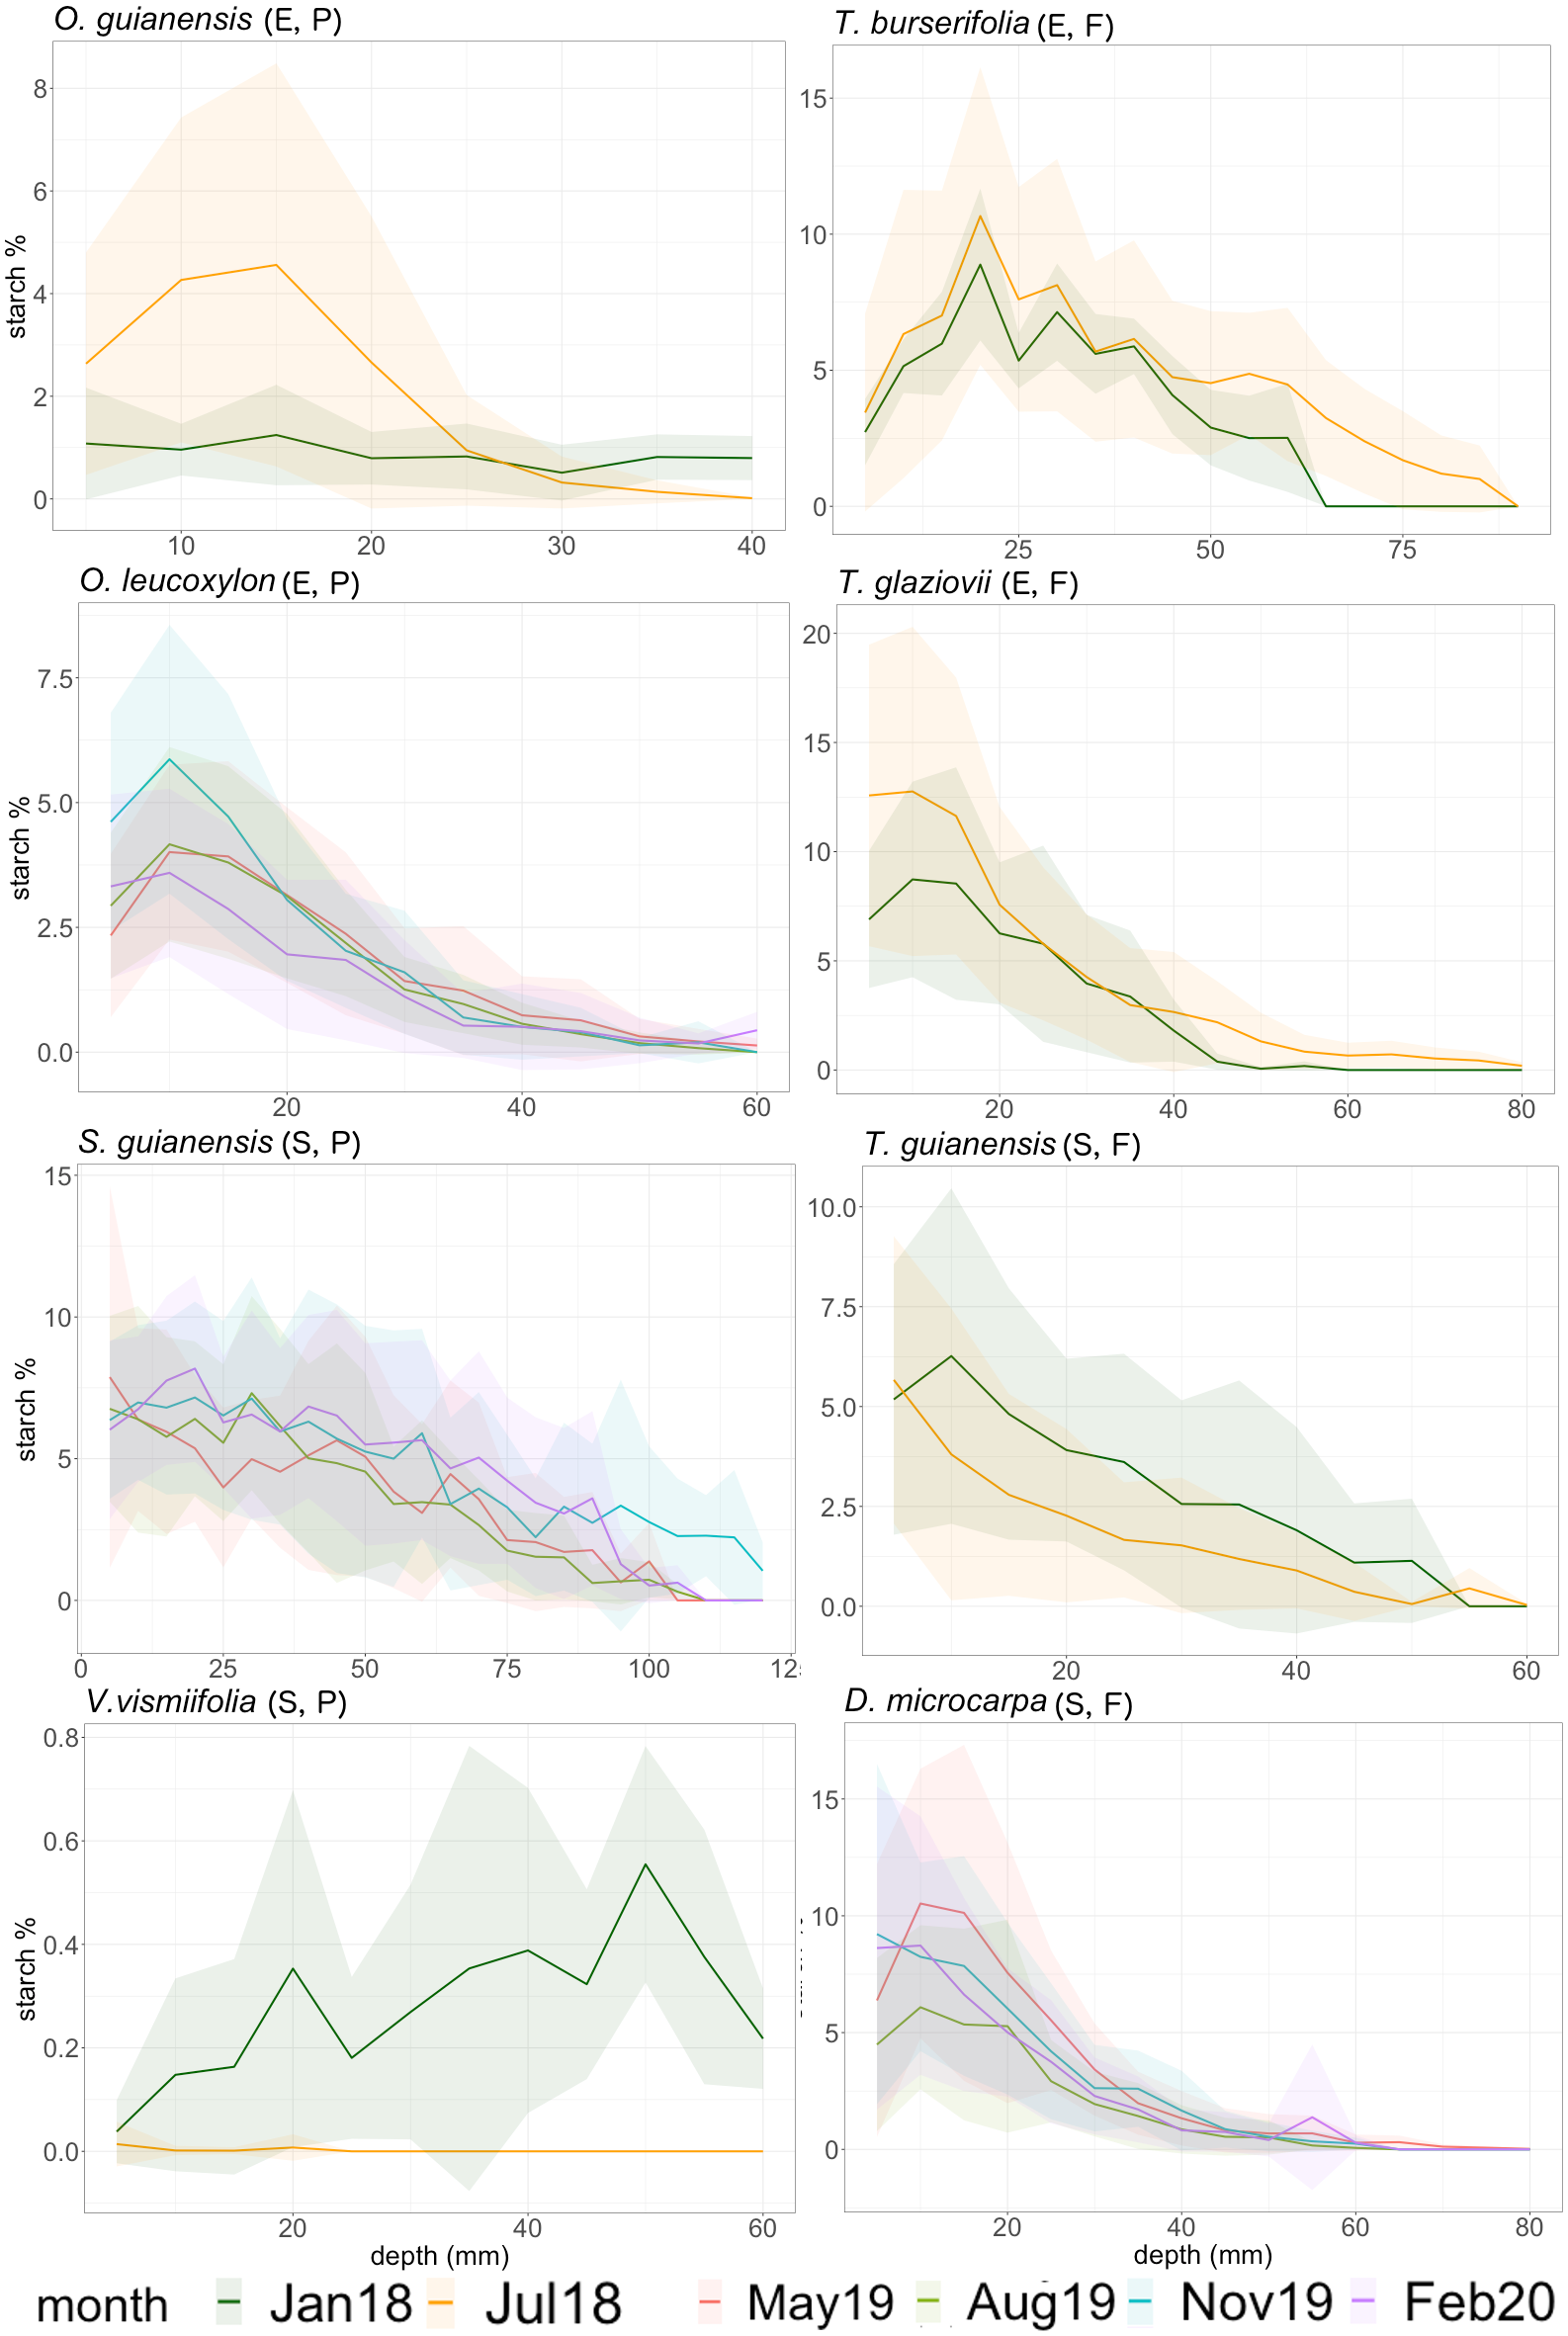
\includegraphics[width=4.5in]{Fig1_radial_concentration_starch.png} 
   \caption{Mean starch concentration (solid lines) and the standard deviation (shaded areas) in the wood of the 8 species evaluated at different wood depths from bark inwards. For \textit{O. leucoxylon, S. guianensis} and \textit{D. microcarpa} we are only showing the lines from the 2019 measurements to avoid confusion. The results of the nonlinear model (equation \ref{starch_area_nlm}) adjusted to each species with the sampling date (month) as a random variable are shown in Table \ref{Nonlinear_mix_models}. In the right hand side are the Fiber storing species (F) and in the left hand side are the parenchyma storing species (P), the first four panels correspond to evergreen species (E) and the last four panels correspond to the semi-deciduous species (S).}
   \label{fig:starch_radial_pattern}
\end{figure}
 
 
Seasonal changes in the radial pattern of starch concentrations were driven mainly by changes in the first 2 cm of wood (Fig. \ref{fig:starch_radial_activity}, upper panel). Nevertheless, relative changes in the starch content, with respect to the maximum starch content measured in 2019, were larger in deeper layers of wood, reaching 100\% towards the limits of the depth distribution of starch (Fig. \ref{fig:starch_radial_activity} lower panel). We did not detect a significant effect of the storage strategy in the seasonal changes of the radial pattern of starch concentrations (p=0.10), but there were significant differences across species (p=0.01) and across leaf habits (pval $< $0.001). The biggest changes in starch concentration between months, during 2019, were observed for semi-deciduous \textit{D. microcarpa} trees (Fig. \ref{fig:starch_radial_activity}) while evergreen species showed less seasonal variation. 



 \begin{figure}[h] %  figure placement: here, top, bottom, or page
   \centering
   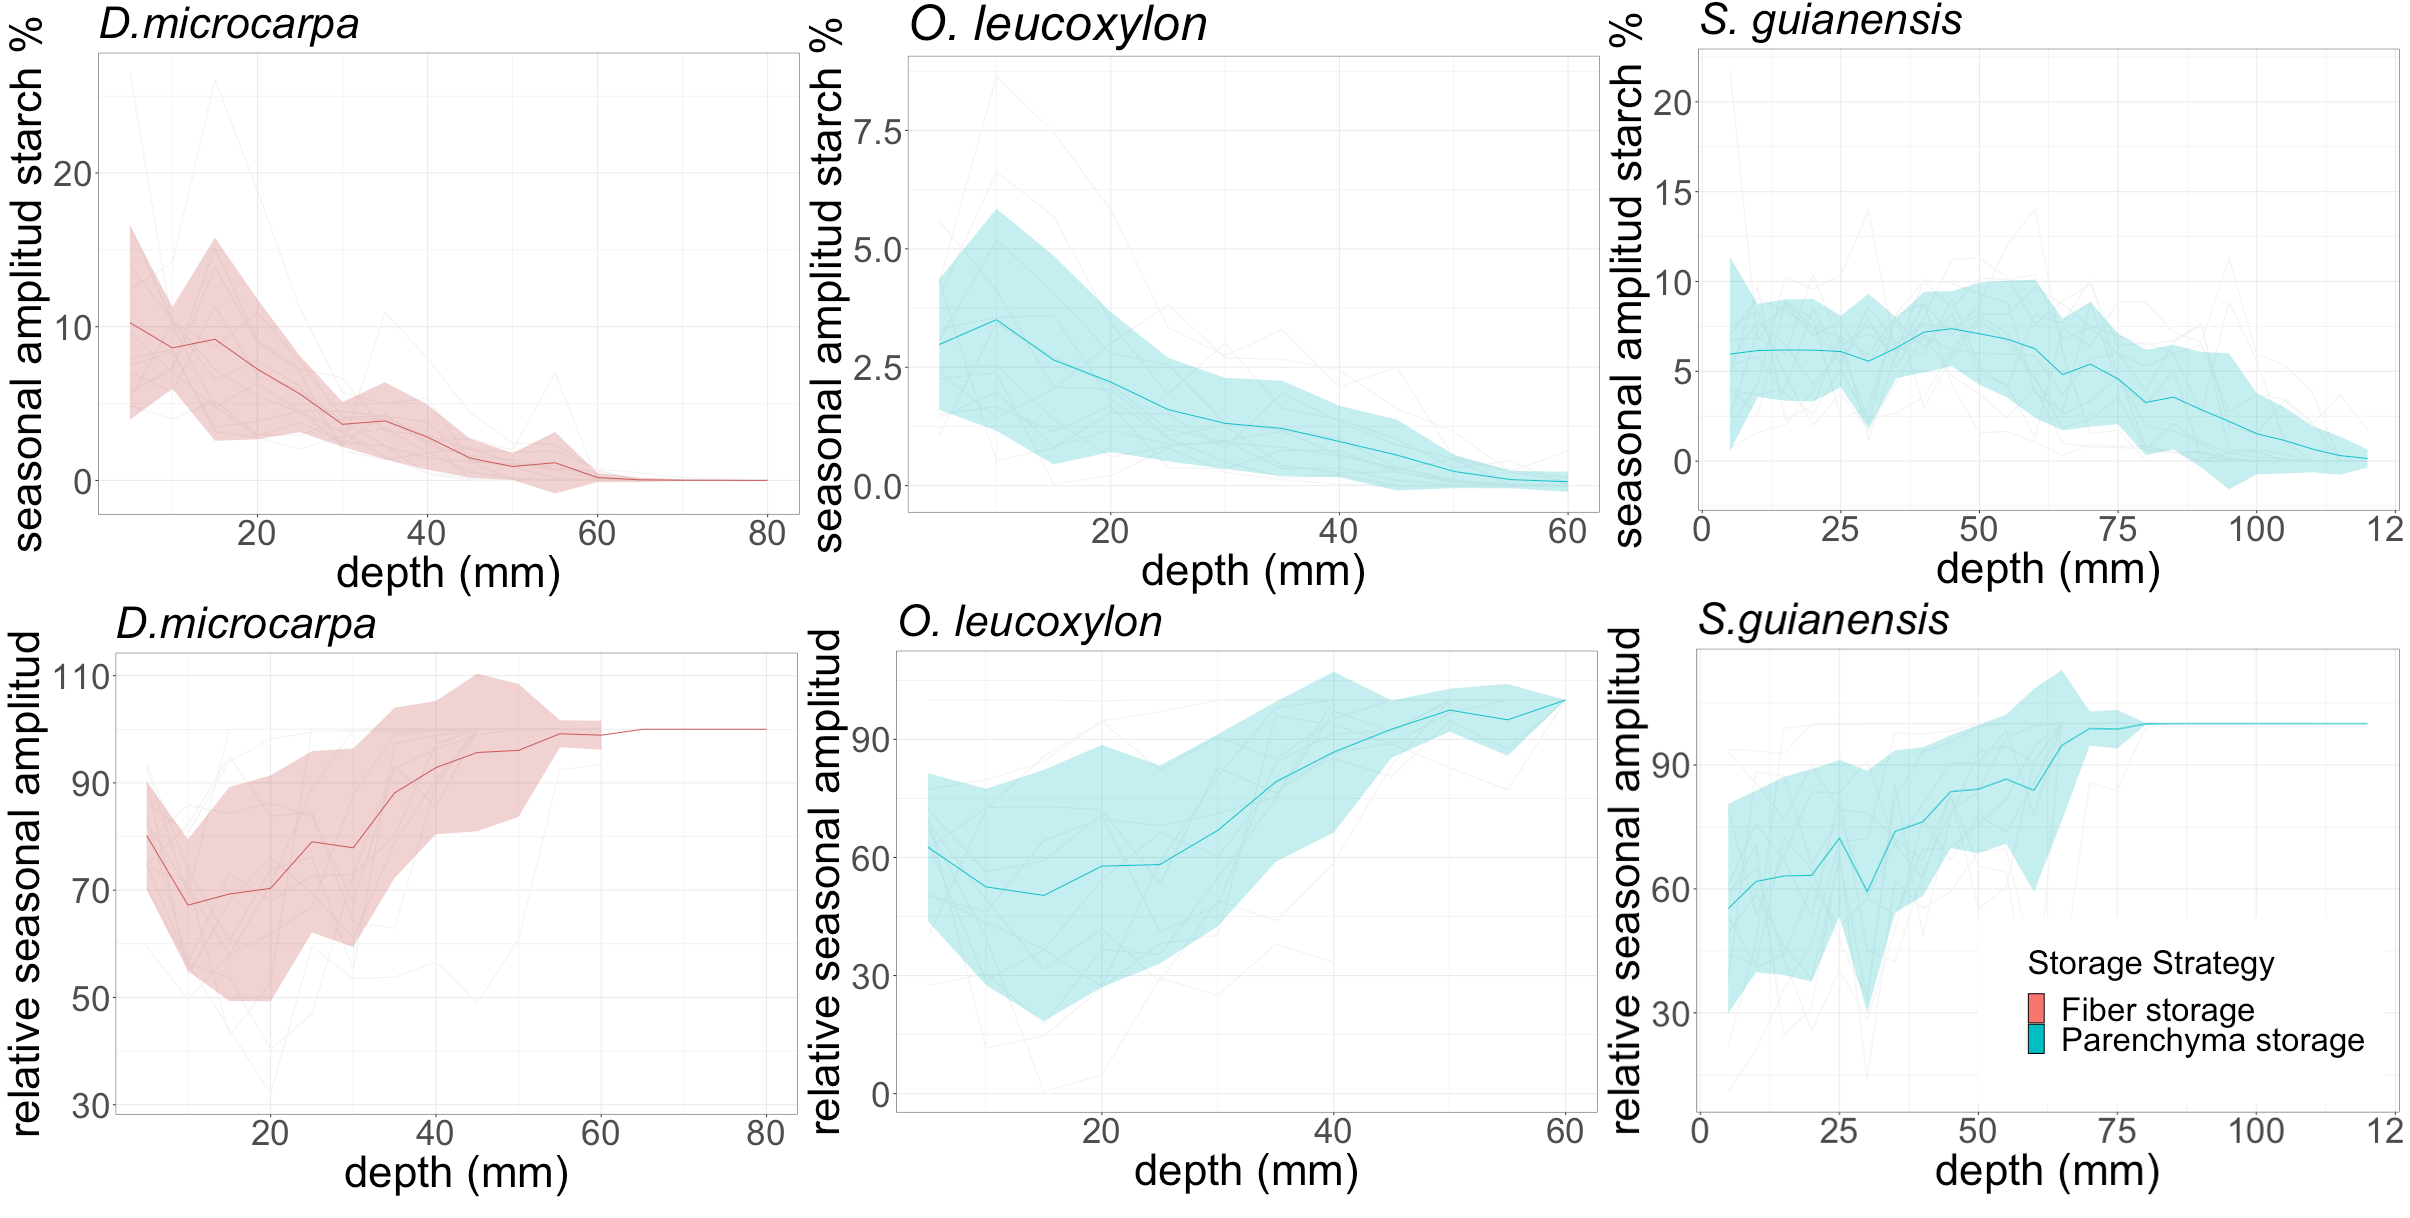
\includegraphics[width=5.5in]{Figure3.png} 
   \caption{Radial metabolic activity of starch in the three species studied during 2019. Upper panels: The metabolic activity measured as the changes in the concentration of starch between months with the maximum and minimum starch content measured during 2019, along the radial profile of wood every 5 mm. The black line is the average difference of starch concentration between seasons and the shaded area represents the standard deviation associated with the individual trees. Lower panels: The relative seasonal  changes of starch in each 5 mm segment of wood with respect to the maximum concentration of starch from the measurements of 2019. The grey shaded areas represent the standard deviation associated with the measured individuals.}
   \label{fig:starch_radial_activity}
\end{figure}


We estimated starch content in the stem wood cores by summing all the concentrations of each 5 mm segment along each wood core. Despite the trends shown in Fig. \ref{fig:starch_radial_activity}, we did not see a significant effect of the sampling date in the estimations of the starch content in any of the evaluated species (Fig. \ref{fig:seasonal_starch_content}). Nevertheless, we found a marginal significant effect of the storage strategy (p=0.055) and leaf habit (p=0.08) on the starch content in the wood, and we saw significant differences between species (p$<$0.001). Semi-deciduous trees of \textit{S. guianensis} had larger starch content in the wood core than the rest of the species, followed by semi-deciduous \textit{D. microcarpa}, and evergreen \textit{T. buserifolia} and \textit{T. glaziovii} trees (Fig. \ref{fig:seasonal_starch_content}). Soluble sugars also showed a decreasing radial pattern in their concentration across sapwood, but we did not find significant differences in the soluble sugar concentrations between the wet and dry season of 2018 for any of the 8 species evaluated (Fig. S3).



\subsection{ Age of the NSC stored in the trees}

We detected a significant effect of the wood age in the $\delta^{14}$C of the soluble carbon and starch. Nonstructural carbon stored deep in old layers of wood had higher $\delta^{14}$C values than NSC stored in new shallow layers of wood, which indicated a pattern of increasing age of NSC with wood age and depth (Fig. \ref{fig:wood_Age_sugar_age}). We did not find differences in the $^{14}$C age of the soluble carbon or starch between species (p=0.6), but we found a marginal effect of the storage strategy on the sugars age (p=0.08, Fig. \ref{fig:D14C_starch}). We observed that individuals that store starch in the fibers seemed to have older NSC than individuals that store starch in the parenchyma (Fig. \ref{fig:D14C_starch}).



\begin{figure}[h] %  figure placement: here, top, bottom, or page
   \centering
   \begin{subfigure}{0.7\textwidth}
   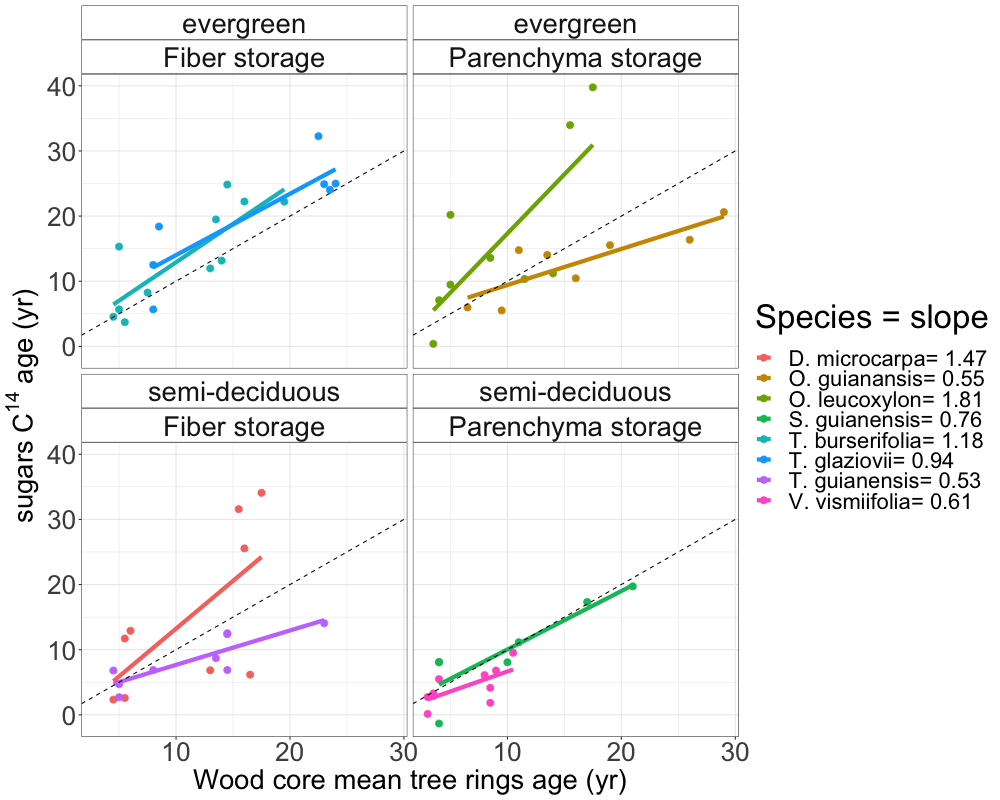
\includegraphics[width=\textwidth]{means_Age_wood_vs_mean_age_sugars_leaf_habit.png} 
   	\caption{Measurements taken in July 2018}
          \label{fig:Jul18} 
       \end{subfigure}
	 \begin{subfigure}{0.7\textwidth}
   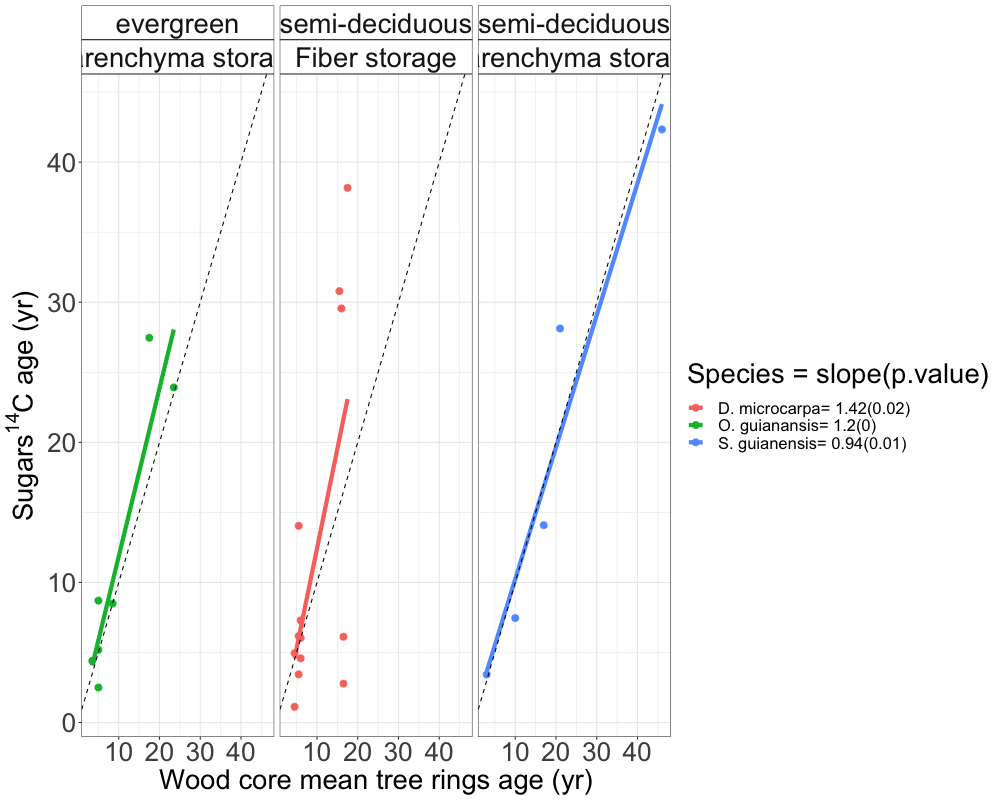
\includegraphics[width=\textwidth]{means_Age_wood_vs_mean_age_sugars_leaf_habit_may2019.png} 
   	\caption{Measurements taken in May 2019}
          	\label{fig:May19} NSC
	\end{subfigure}
   \caption{Comparison between the sugars $^{14}$C mean age and the wood core mean age estimated by counting annual tree rings. Dashed lines represent the 1:1 ratio between the two mean ages. }
   \label{fig:wood_Age_sugar_age}
\end{figure}	


Regression lines between the average $^{14}$C age of the soluble carbon in wood and the average age of wood (estimated by ring counting) per species, for July 2018 indicated how fast tree species may cycle their reserves and the predominant direction of radial mixing of NSC in wood during that time of the year (Fig. \ref{fig:wood_Age_sugar_age}). Regression slopes bigger than one and intercepts bigger than zero indicated that NSC was older than the wood containing it, and therefore very slow NSC cycling rates and predominantly outward mixing of NSC from deep old layers of wood to new ones during this sampling date. Despite no significant differences between groups, we observed that evergreen fiber-storing species had older NSC than the associated wood; and semi-deciduous parenchyma-storing species had NSC younger than the wood containing it. The other two groups showed a combination of the two scenarios (Fig. \ref{fig:wood_Age_sugar_age}). We found a weak but significant correlation between the annual growth rate of the wood and the $^{14}$C age of the NSC standardised by the age of the wood (p=0.045, Figure S5), this indicates that slow growing trees store carbon for long periods of time and tend to have outward mixing of very old NSC to maintain NSC supply when the demand of carbon is higher than the supply.

Soluble carbon and starch from the stem wood cores had, in general, similar $\delta^{14}$C signature (Fig. S6). For a couple of individuals starch had larger $\delta^{14}$C values than the soluble carbon, indicating that starch may be older than the soluble carbon for these few trees. Unfortunately, we lost most of the starch measurements during the analysis. From those remaining samples, we had to discard samples that had a sugar/enzyme ratio lower than 0.5 (resulting from the starch extraction procedure), because the model used for corrections (Equation \ref{starch_mass_balance_eq}) was not calibrated for these values and the correction of these measurements was not reliable. Then, we show the comparison for 7 reliable measurements (Fig. S6). 


 \begin{figure}[h] %  figure placement: here, top, bottom, or page
   \centering
   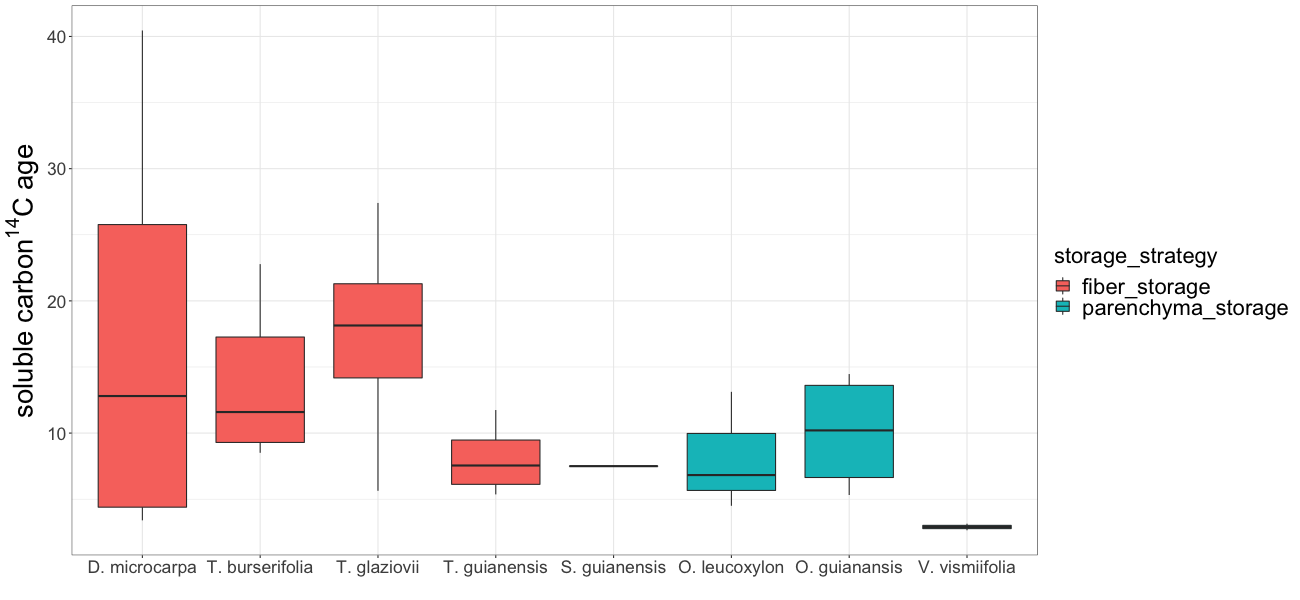
\includegraphics[width=5.5in]{D14C_sugars_perspecies.png} 
   \caption{ Soluble carbon $\delta^1{14}$C boxplot for each species studied divided between fiber storing and parenchyma storing species. The black line inside the boxplot shows the median; the upper and lower limits of the filled area correspond to the 75th and 25th quartiles of the distribution respectively.}
   \label{fig:D14C_starch}
\end{figure}
 

\subsection{Age of the respired CO$_2$}

The respired CO$_{2}$ from the wood cores was on average 5 years older than the atmospheric CO$_{2}$, based on $^{14}$C estimations for all the species. The $\delta^{14}$C of the emitted CO$_{2}$ was slightly higher than the one corresponding to the carbon fixed in 2019, evidencing the contribution of old carbon to respiration (Fig. \ref{fig:D14_CO2}). Nevertheless, it was also significantly lower than the $\delta^{14}$C of the NSC reserves in the first 4 cm of each wood core (Fig. \ref{fig:NSC_D14_CO2}). We did not observe differences between species in the $\delta^{14}$C of the respired CO$_{2}$ from the wood cores in May 2019 (Fig. \ref{fig:D14_CO2}). For \textit{D. microcarpa} we observed a higher $\delta^{14}$C of the respired CO$_{2}$ during the dry season of 2018 (July) with respect to the wet season of 2019 (May, Fig. \ref{fig:NSC_D14_CO2}). We found a negative relationship between the $\delta^{14}$C of the emitted CO$_{2}$ and the trees' annual wood growth rates and a positive relationship between the $\delta^{14}$C of the emitted CO$_{2}$ and the number of tree rings in each wood core (Fig. S7).


 \begin{figure}[ht] %  figure placement: here, top, bottom, or page
   \centering
   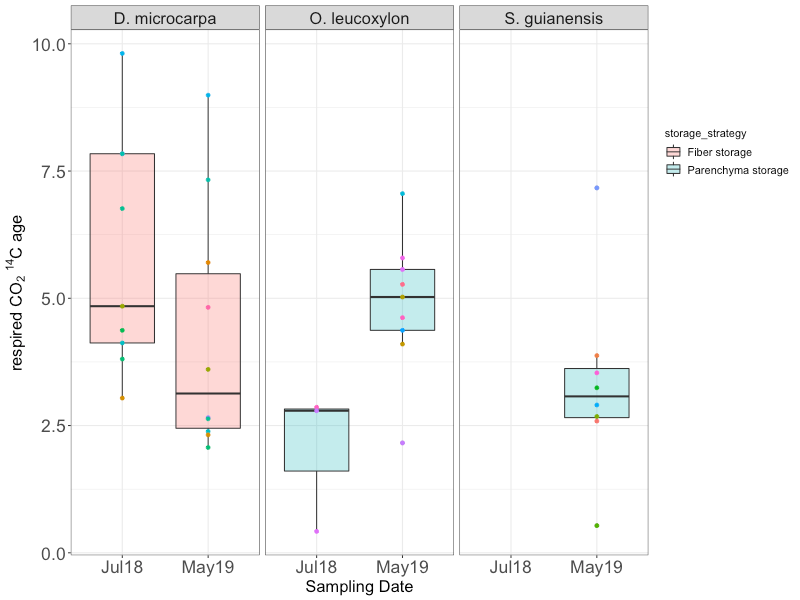
\includegraphics[width=5.5in]{resp_CO2_ges.png} 
   \caption{ $\delta^{14}$C of the respired CO$_2$ directly by the wood cores from trees sampled in may 2019.}
   \label{fig:D14_CO2}
\end{figure}


% \begin{figure}[ht] %  figure placement: here, top, bottom, or page
%   \centering
%   \includegraphics[width=5in]{NSC_D14C_CO2_D_micro.png} 
%   \caption{ Comparison between the $^{14}$C of the NSC stored in the wood cores and the CO$_2$ emitted by that wood core from individuals of \textit{D.microcarpa}. The solid line represents the 1:1 line and serves as a reference for the relationship. The data points under the 1:1 line indicate that the NSC stored in the wood  is much older than the carbon being respired by the wood.  
%}
%   \label{fig:NSC_D14_CO2}
%\end{figure}



\section{Discussion}

\subsection{ Seasonality of NSC}

Our results confirm significant seasonality of starch concentrations across different wood depths and slight seasonal changes of the starch content in the wood across a set of tropical species in a seasonal dry forest in Brazil. Notably, we observed that for some of these trees the seasonal variation of the starch content across wood was maintained by a strong outward mixing of old NSC from inner layers of sapwood to outer ones, which made the NSC to look older than the wood that contained them during the dry season of July 2018. We expected the storage strategy of starch in the wood and leaf habit to influence the seasonal fluctuation of starch across sapwood depths. Contrary to our hypothesis, we did not observe a clear relationship between seasonal changes in starch content and the storage strategy of starch in wood or leaf habit. Nevertheless, during 2019 we observed the largest seasonal changes in starch concentrations across all sapwood depths for \textit{D. microcarpa}, a fiber storing species, while for the other two parenchyma storing species \textit{S. guianensis} and \textit{O. leucoxylon} the seasonal fluctuations of starch concentrations were smaller. This suggests that fiber storing species could have slightly larger seasonal fluctuations of starch concentration at each wood depth than parenchyma storing species, and indicates that starch storage in wood living fibers may not limit starch mobilisation and use across wood as previously thought \citep{Herrera-remirez:2021}. There might be other physiological and anatomical traits such as size and distribution of parenchyma cells, longevity of living wood cells and porosity size, that determine the radial distribution of starch and its seasonal activity for tropical trees. Future work should expand on tree species and functional traits to clarify the mechanistic controls of these patterns.

The decline of NSC concentration with increasing sapwood depth has been already reported for many species \citep{fischer:1991, Barbaroux:2002, Hoch:2003, Richardson:2015, Fuze2020}, including tropical trees \citep{Newell:2002, Wurth:2005}. The seasonal changes of the starch concentration at all sapwood depths, found in this study, support recent results indicating that starch reserves are metabolically active all across the sapwood, and starch from all depth ranges contributes to metabolism \citep{Trumbore:2015, Fuze2020}. We observed that although changes in the deeper sapwood layers were small in absolute terms, the relative change reached 100\% for all trees investigated. This, along with the fact that deeper layers of wood were completely devoid of starch, suggest that these tropical trees are able to completely remobilize the starch stored in deep wood layers when it is needed to regulate metabolism. Therefore, carbon seemed to not be permanently sequestered as starch in wood, remaining always accessible for usage.

These seasonal changes in starch content were likely responding to the imbalance between carbon sources and sinks. These imbalances might have been induced by seasonal changes in precipitation and relative humidity at the site. Intriguingly, the seasonal fluctuation in starch content contrasted between the years 2018 and 2019. In 2018 starch content peaked during the dry season and decreased during the wet season, for most of the species (Fig. \ref{fig:seasonal_starch_content}). This suggests that during 2018 the NSC content might have been controlled by reductions in dry season sink activity, where growth and respiration decreased more than photosynthesis. It has been commonly reported that under moderate stressful conditions such as water shortage, low temperature and nutrient deficiency, growth and respiration are down regulated more rapidly and severely than photosynthesis  \citep{Hoch:2003ui, Korner:2003, Wurth:2005, Hartmann:2015}. Nevertheless, \citet{Obrien:2015} suggested that depending on the severity of the stress the control of the NSC dynamics may shift from sink activity to source activity. They reported that during mild drought conditions the source activity of tropical seedlings gets more affected than sink activity, leading to a decrease in the NSC content. Our results are in agreement with the ones reported by \citet{Obrien:2015}, suggesting that this shift between sink activity and source activity control over the NSC changes may also apply to adult tropical trees. Alternatively, trees should have simply stored more starch during the dry season prioritizing storage over growth and respiration \citep{Huan:2019}. In 2019 we observed that starch content peaked during the beginning or the end of the wet season and fell during the dry season. This suggests that during 2019 NSC content may have been controlled by source activity. Growth and respiration in all three species might have been not strongly affected throughout 2019 where NSC reserves might have regulated it (Fig. S8). Photosynthesis may have been strongly affected during the dry season, as suggested by the strong decrease in the sap flow and the massive loss of mature leaves from July to September (Fig. S9). Among the three species evaluated, \textit{D. microcarpa} showed the bigger changes in mature leaf coverage and sap flow, and it showed the higher wood respiration rates. This may explain why \textit{D. microcarpa} trees had the larger seasonal fluctuations in starch concentration across the wood, suggesting that a larger number of living fibers, which increase the volume of living wood, increase the respiratory requirements. This may push trees to invest more carbon in maintaining higher quantities of NSC in wood to support a regular high active metabolism, which may increase survival at expenses of growth.


\subsection{NSC age, lateral mixing and use}

Our results add to published studies that have reported that NSC reserves in tree stems can be decades old \citep{carbone:2007, carbone:2013, muhr:2013,muhr:2016, Muhr:2018, Richardson:2013aa, Trumbore:2015}. Furthermore, we found that the estimated age of the NSC is positively related to wood age, causing NSC age to increase with wood depth. This is in agreement with previous studies that reported similar patterns of the age of the NSC in stem wood in temperate trees \citep{Richardson:2015, Trumbore:2015, Fuze2020}. We did not find significant differences between storage strategies or leaf habits in terms of $\delta^{14}$C of the NSC. Nevertheless, fiber storing trees tended to have higher $^{14}$C ages of the NSC than parenchyma storing species (p=0.076). Differences in the age of the NSC in temperate trees has been found in species with different leaf habit or growth strategies  \citep{Richardson:2015, Richardson:2013aa}. Deciduous trees have been found to be more conservative in the use of their reserves and therefore showed larger and older NSC reserves pools than evergreen species \citep{Trumbore:2015}. Similarly, slow growing species tend to store NSC for longer times, resulting in older and larger NSC than fast growing species \citep{Richardson:2013aa}. This is consistent with our results where slow growing, fiber storing, trees tended to have higher $\delta^{14}$C of NSC and larger NSC reserves.

We observed that some of these slow growing trees had a higher $^{14}$C age of NSC than the age of the containing wood at the same depth, indicating that this NSC was fixed before the wood containing it was constructed. To our knowledge, this is the first time that this pattern has been observed in trees. Surprisingly, some of these species also showed high seasonal changes in the NSC content across wood depths, but seasonal changes in wood starch content all over the wood core were smaller. This may be explained by an outward mixing of very old NSC from deep layers of wood towards the cambium during the dry season of 2018 which might have dramatically increased the mean age of the NSC stored in wood during this period of time for some trees with very old storage. Nevertheless, alternative explanations should also be considered for the presence of soluble carbon older than the containing wood at any depth: i) there might be an influx of older NSC from other tree organs like roots \citep{klein:2015, Herrera-Ramirez:2020}; ii) constant and rapid interconversion between starch and other compounds such as lipids, sugars or other organic compounds that may be older than the containing wood  \citep{Richardson:2015}; and iii) refixation of large amounts of respired CO$_{2}$ into the NSC pools \citep{Bloemen:2013, Hilman:2019}. During the productive season, where NSC content increases, we might expect that these NSC ages decrease because of the influx of new NSC from the phloem \citep{Dandrea:2019}, during this period NSC age might turn lower than the wood age. 
 
We also observed trees that had a lower $^{14}$C age of NSC than the age of the wood that contained it, indicating that for these trees NSC concentrations were maintained by a strong inward mixing of young NSC. This pattern has been already reported for several temperate species \citep{Richardson:2015, Trumbore:2015, Fuze2020}. Interestingly, there appears to exist a pattern in our data, though not statistically significant, between the NSC age composition, the storage strategies, the leaf habit and the predominant direction of lateral mixing of NSC during the dry season of 2018. Semi-deciduous trees that store starch in the parenchyma had predominantly young NSC and inward mixing of young NSC towards deep wood layers; while evergreen fiber storing trees usually had predominantly old stored NSC and outward mixing of old NSC toward shallow wood layers. Variability in inward mixing has been reported before and associated with wood anatomy and life traits  \citep{Richardson:2015, Trumbore:2015}. These studies have reported stronger mixing-in in temperate, evergreen, diffuse-porous, softwood (Pinus strobus L.) trees compared with deciduous, ring-porous, hardwood (Quercus rubra) trees. Additionally, these differences in lateral mixing rates may also be expected with differences in carbon allocation patterns, water regulation and growth \citep{mcdowell:2008, carbone:2013, Hartmann:2015}. Our results suggest that for the tropical species we studied the storage strategy of starch in wood, leaf habit and growth rates may be a good indicator of the strength and direction of the NSC lateral mixing in wood during periods that the stored NSC has to be remobilized.

\subsection{$\delta^{14}$C of the CO$_2$ emitted by wood cores}

The collected wood cores from the three species studied in 2019 respired CO$_{2}$ on average 5 years older than recent assimilates. This confirms previous results that show the contribution of stored old NSC to respiration \citep{Varga:2009, carbone:2013,  muhr:2013, Trumbore:2015}. We did not observe differences in the $\delta^{14}$C of the emitted CO$_{2}$ from the wood cores among species, which contrasts with what has been previously reported for Quercus trees, where growth rates and leaf habit had an effect on the $\delta^{14}$C of the CO$_{2}$ emitted by tree stems  \citep{Trumbore:2015}. Nevertheless, differences between the emitted CO$_{2}$ directly from the wood core and the emitted CO$_{2}$ by tree stems probably reflect post respiration processes such as CO$_{2}$ refixation and vertical transport inside tree stems \citep{muhr:2013}.

Although there is a contribution of old NSC to wood respiration, we observed that the CO$_{2}$ efflux from the incubated wood cores was still composed of significantly younger carbon than the stored NSC for all species evaluated. Additionally, the excellent correspondence of $^{14}$C ages and dendrochronological ages for all but one of our species indicates that the structural C is built of recently fixed C. This indicates that the transit time of the NSC of these healthy trees is mainly composed of younger carbon. Similar results have been reported by measurements and simulations of respired CO$_{2}$ age in temperate species, which suggest that the respired CO$_{2}$ is a mixture of ages composed mainly of young carbon when trees are not C limited  \citep{muhr:2013, Richardson:2015, ceballos_nunez:2018, Herrera-Ramirez:2020}. When trees experience a stress or disturbance that limits carbon assimilation and depletes the NSC reserves, the $\delta^{14}$C of CO$_{2}$ increases because an increasing contribution of older NSC to sustain metabolism \citep{Herrera-Ramirez:2020, Richardson:2013aa, Muhr:2018}. This was in agreement with our observations from different seasons. Despite we did not find statistical significance in the comparison between seasons, we observed a higher $\delta^{14}$C in the CO$_{2}$ respired in July 18 (dry season) than in May 19 (wet season) when the starch content in wood increased for \textit{D. microcarpa}, and we observed lower $\delta^{14}$C in the CO$_{2}$ respired in July 18 (dry season) than in May 19 (wet season) when the starch content slightly decreased for some individuals of \textit{O. leucoxylon}. Unfortunately the loss of samples from July 2018 impaired us to evaluate this change in \textit{S. guianensis}. This indicates the use of a higher proportion of old stored NSC to regulate metabolism during the dry season 2018 than during the wet season 2019 for \textit{D. microcarpa} trees, and probably the contrary happened for some \textit{O. leucoxylon} trees. These changes in the transit time of the NSC can reflect the existence of different NSC pools in the wood with different cycling rates (such as storage in deeper layer of wood and in outer layers of wood, or storage in the wood living fibers vs storage in the parenchyma cells), and the asymmetric distribution of NSC age in each of those pools \citep{Herrera-Ramirez:2020}. This also demonstrates the utility of measuring and estimating mean transit times (age of the respired CO$_{2}$ and C allocated to growth) as indicative of the degree of storage utilization and probably the degree of tree stress under certain environmental conditions.

\subsection{Conclusions}

By using wood histological methods for starch quantification and radiocarbon analysis, we provide insights into the radial distribution of starch in wood, its seasonal fluctuations, the internal radial mixing dynamics and the mean age and transit time of NSC in wood within trees with contrasting wood functional traits. Our measurements show that NSC is metabolically active all across the sapwood depth and that fiber storing trees might have higher metabolic activity than parenchyma storing trees. Most importantly, these highly metabolically active trees hold carbon in wood for decades and maintain the NSC radial concentration across sapwood by a predominantly outward mixing of old NSC from old deep layers of wood to young shallow layers of wood. This mixing caused the age of NSC at a given sapwood depth to be higher than the age of wood, at least during the dry season. Furthermore, despite this very old NSC stored in the wood, trees respired significantly younger CO$_{2}$, although not as young as current year assimilates. Interestingly, this age of the respired CO$_{2}$ increased during the dry season of 2019 due to the use of older NSC reserves stored in the wood. These changes in transit time of NSC helped us to understand how much of the reserves were used by trees under carbon shortages, and may give an indication about the resilience of trees to stressful conditions. Further research should point in this direction.

\bibliographystyle{frontiersinSCNS_ENG_HUMS}
\bibliography{NSC_seasonality} 



 
\end{document}







